% % % % % % % % % % % % % % % % % % % % % % % % % % % % % % % % % % % % % % % % % % % %
%                                                                                     %
% Short Sectioned Assignment LaTeX Template Version 1.0 (5/5/12)                      %
% This template has been downloaded from: http://www.LaTeXTemplates.com               %
%                                                                                     %
% Original author:  Frits Wenneker (http://www.howtotex.com)                          %
%                                                                                     %
% Modified by: Fco Javier Sueza Rodríguez (fcosueza@disroot.org)                      %
%                                                                                     %
% Changes:                                                                            %
%	    - Custom Chapters, Sections and Subsections (titlesec package)                %
%           - Document type scrbook (oneside)                                         %
%           - Use babel-lang-spanish package and marvosym                             %
%           - Use hyperref, enumitem, tcolorbox and glossaries packages               %
%           - Use Time New Roman (mathptmx), Helvetic and Courier fonts               %
%                                                                                     %
% License: CC BY-NC-SA 3.0 (http://creativecommons.org/licenses/by-nc-sa/3.0/)        %
%                                                                                     %
% % % % % % % % % % % % % % % % % % % % % % % % % % % % % % % % % % % % % % % % % % % %

%-----------------------------------------------%
%	              Packages                  %
%-----------------------------------------------%

\documentclass[paper=a4, fontsize=11pt, oneside]{scrbook}

% ---- Text Input/Output ----- %

\usepackage[T1]{fontenc}
\usepackage[utf8]{inputenc}
\usepackage{mathptmx}
\usepackage[scaled=.92]{helvet}
\usepackage{courier}
\usepackage[indent=12pt]{parskip}

\usepackage{geometry}
\geometry{verbose,tmargin=3cm,bmargin=3cm,lmargin=2.6cm,rmargin=2.6cm}

% ---- Language ----- %

\usepackage[spanish]{babel}
\usepackage{marvosym}

% ---- Another packages ---- %

\usepackage{amsmath,amsfonts,amsthm}
\usepackage{graphics,graphicx}
\usepackage{titlesec}
\usepackage{fancyhdr}
\usepackage{tcolorbox}
\usepackage{hyperref}
\usepackage{enumitem}
\usepackage[automake]{glossaries}

%--------------------------------------------------------------------%
%                      Customizing Document                          %
%--------------------------------------------------------------------%


% ----------- Custom Chapters, Sections and Subsections -------------- %

\titleformat{\chapter}[display]
			{\bfseries\Huge}
			{Tema \ \thechapter} {0.5ex}
			{\vspace{1ex}\centering}

\titleformat{\section}[hang]
			{\bfseries\Large}
			{\thesection}{0.5em}{}

\titleformat{\subsection}[hang]
			{\bfseries\large}
			{\thesubsection}{0.5em}{}

\titleformat{\subsubsection}[hang]
			{\bfseries\large}
			{\thesubsubsection}{0.5em}{}

\hypersetup{
    colorlinks=true,
    linkcolor=black,
    urlcolor=magenta
}

% ------------------- Custom heaaders and footers ------------------- %

\pagestyle{fancyplain}

\fancyhead[]{}
\fancyfoot[L]{}
\fancyfoot[C]{}
\fancyfoot[R]{\thepage}

\renewcommand{\headrulewidth}{0pt} % Remove header underlines
\renewcommand{\footrulewidth}{0pt} % Remove footer underlines

\setlength{\headheight}{13.6pt} % Customize the height of the header

% --------- Numbering equations, figures and tables ----------------- %

\numberwithin{equation}{section} % Number equations within sections
\numberwithin{figure}{section} % Number figures within sections
\numberwithin{table}{section} % Number tables within sections

% ------------------------ New Commands ----------------------------- %

\newcommand{\horrule}[1]{\rule{\linewidth}{#1}} % Create horizontal rule command


%----------------------------------------------------------------------------------------
%	TÍTULO Y DATOS DEL ALUMNO
%----------------------------------------------------------------------------------------

\title{
\vspace{10ex}
\normalfont \normalsize
\huge \textbf{Tarea 1: La Empresa y su Clasificación}
}
\author{Francisco Javier Sueza Rodríguez}
\date{\normalsize\today}

%----------------------------------------------------------------------------------------
%                                     DOCUMENTO
%----------------------------------------------------------------------------------------
\begin{document}

\maketitle

\thispagestyle{empty}

\vspace{75ex}

\begin{center}
    \begin{tabular}{l l}
        \textbf{Centro}: & IES Aguadulce \\
        \textbf{Ciclo Formativo}: & Desarrollo Aplicaciones Web (Distancia)\\
        \textbf{Asignatura}: & Empresa e Iniciativa Emprendedora\\
        \textbf{Tema}: & Tema 1 -  La Empresa y su Clasificación\\
    \end{tabular}
\end{center}

\newpage

\section{Actividad 1: Elige una Empresa}

\subsection{Enunciado}
Imaginaos, es la empresa que eligió Claudia para ejemplificar los contenidos de la unidad 1, ahora te proponemos que seas tú el que elija una empresa en la que apliques lo que hemos estudiado. Los motivos de esta elección pueden ser los que quieras: trabajas en ella, te gustaría formar parte de su plantilla o haberla creado, está relacionada con el ciclo formativo que cursas, es de tu localidad o has leído sobre ella y te gusta su organización, porque es muy rentable, por la forma de contratar y de crear equipos, por su originalidad y creatividad, porque es socialmente responsable…

Responde a estos tres apartados en no más de 10 líneas.

\begin{enumerate}[label=\roman*.]
    \item El nombre de la empresa y el motivo por el que la has elegido.
    \item Actividad que realiza: ¿qué necesidades satisface en el mercado? ¿Produce bienes y/o presta servicios?
    \item En esta tarea te pedimos que elijas tú una empresa y hagas lo mismo que Claudia.
\end{enumerate}

\subsection{Solución}
\begin{enumerate}[label=\roman*.]
    \item La empresa que he elegido es \textbf{Urban Green Club}, una Startup que se dedica a la implantación y mejora de huertos urbanos, motivo por el cual \textbf{la he elegido}, ya que me parece que es una actividad bastante interesante.

    \item La empresa se dedica al \textbf{asesoramiento y creación de huertos urbanos} y la concienciación medioambiental. En este aspecto es una empresa que \textbf{presta servicios} para cubrir la \textbf{necesidad} de la gente de estar en contacto con la naturaleza en medios urbanos y de cultivar su propia fruta y verdura.

    \item Entre sus clientes se encuentra tanto \textbf{ayuntamientos} como \textbf{particulares}, siendo una de las \textbf{principales características} de ambos tener cierta concienciación sobre la sostenibilidad y la necesitad de crear espacios verdes en las grandes ciudades que permitan mantener cierto contacto con la naturaleza.
\end{enumerate}

\section{Actividad 2: Indica sus Elementos}

\subsection{Enunciado}
Identifica los elementos de la empresa que has elegido en la actividad 1 siguiendo la clasificación establecida en la unidad: Elementos humanos, elementos materiales y organización.

\subsection{Solución}
Los principales \textbf{elementos} que podemos encontrar en la empresa \textbf{Urban Green Club} son los siguientes:

\begin{itemize}
    \item \textbf{Elementos Humano}: en esta empresa los elementos humanos están compuesto por la \textbf{CEO} o la directora ejecutiva, y por el resto de empleados. En este caso hay \textbf{empleados dedicados} al \textbf{marketing} de la empresa, al \textbf{asesoramiento técnico} sobre la implantación de los huertos, a la \textbf{gestión de proyectos}.

    \item \textbf{Elementos Materiales}: ya que la empresa se dedica a la creación y mejora de huertos urbanos deberá tener materiales para dicho fin, como diferentes tipos de abonos, plantas, fertilizantes, elementos para el riego, herramientas para realizar la plantación, etc.. Además, deberán tener equipos informáticos para buscar información, llevar a cabo labores de marketing, establecer contacto con clientes, etc. También deberá tener un local para desarrollar su actividad, en este caso, está en el Centro de Iniciativas Empresariales de Granada.

    \item \textbf{Elementos de Organización}: hay diferentes elementos de organización en esta empresa, ya que hay que \textbf{organizar las laboras de marketing}, algo fundamental para dar a conocer. Además, los \textbf{proyectos de huerto urbano} necesitan una \textbf{buena organización} para que sean productivos y no se desperdicien elementos materiales, especialmente en esta empresa que tiene la sostenibilidad por bandera. Por lo que habrá que organizar la adquisición de materiales para los huertos así como usarlos de la forma más eficiente posible adaptándolos a los requisitos de los clientes.
\end{itemize}

\section{Actividad 3: Analiza sus Funciones}
\subsection{Enunciado}
En la unidad hay un ejemplo que puede servirte de ayuda para la realización de este apartado de la tarea: ¡Pincha en el dibujo de la fábrica de muebles!.
Te pedimos que determines y describas brevemente las funciones que puede tener la empresa de tu ejemplo. Esta actividad no debe ocupar más de 10 líneas.

Orientaciones: Te recomendamos para ello que sigas los siguientes pasos:

\begin{enumerate}
    \item Identifica posibles tareas que haya que realizar en el negocio.
    \item Agrupa las tareas que sean afines: grupos de tareas.
    \item Identifica con qué función se corresponde cada grupo de tareas.
\end{enumerate}

Recuerda que en los comienzos de una empresa o dependiendo del tipo que sea, no se desarrollen todas las funciones mencionadas en la unidad o unas son más importantes que otras.

\subsection{Solución}
En esta empresa, aunque es una Startup de reciente creación, las funciones están bastante bien delimitadas. La \textbf{función comercial} consistirá en diseñar y administrar la página web de la empresa así como las diferentes acciones publicitarias. La \textbf{función de producción} consistirá en el diseño e implantación de los huertos urbanos adaptados a las exigencias del clientes y realizados de forma sostenible. Para llevar a la cabo la implantación de los huertos de forma eficiente deberá de haber un control de los gastos y beneficios, concretados en al \textbf{función financiare}, que ademas deberá de intentar captar inversión exterior para su rápido crecimiento. La \textbf{función social} la cumplirán los empleados en la diferentes áreas, como marketing, expertos en agronomía, etc.  Por último, la \textbf{función directiva} consistirá en organizar los equipos implicados en todas las funciones anteriores para que trabajen conjuntamente de forma eficiente.

\section{Actividad 4: Clasifica tu Empresa}

\subsection{Enunciado}
Clasifica la empresa que pusiste en la actividad 1 atendiendo a los criterios de clasificación establecidos en el tema:

\begin{itemize}
    \item Sector económico en el que se incluye:
    \item Actividad económica que realiza:
    \item Dimensión o efectivos de personal:
    \item Ámbito geográfico en el que ejerce su actividad:
    \item Titularidad del negocio:
\end{itemize}

\subsection{Solución}
La clasificación de Urban Green Club es la siguiente:

\begin{itemize}
    \item \textbf{Sector económico en el que se incluye}:  es una empresa que se dedica al \textbf{sector terciario}.
    \item \textbf{Actividad económica que realiza}: la actividad económica que realiza según las Clasificación Nacional de Actividades Económicas (CNAE) es la de \textbf{Apoyo a las Actividades de Agricultura} (CNAE 0161) incluida dentro de las empresas de servicios.
    \item \textbf{Dimensión o efectivos de personal}: según el número de trabajadores, es una \textbf{microempresa}, ya que no tiene más de 10 trabajadores.
    \item \textbf{Ámbito geográfico en el que ejerce su actividad}: es una empresa \textbf{local}, ya que solo trabaja en Granada y en pueblos de los alrededores.
    \item \textbf{Titularidad del negocio}: el capital de la empresa es \textbf{privado}, por lo que es una \textbf{empresa privada}.
\end{itemize}

\section{Actividad 5: ¡Eres el Responsable de la Ética de la Empresa!}

\subsection{Enunciado}
Imagina que fueras el empresario o empresaria de la empresa que has seleccionado en la pregunta 1, indica una acción concreta que llevarías a cabo en materia de Responsabilidad Social y que formaría parte de la cultura de tu empresa. Te pedimos que nos digas en no más de 10 líneas:

\begin{enumerate}
    \item El grupo de interés o stackeholders al que va dirigida.
    \item Una descripción de la acción.
    \item Algunos recursos que necesitas para llevarla a cabo: contactos, colaboraciones, dinero, materiales, etc.
    \item Los indicadores que puedes utilizar para valorar si la medida es eficaz.
\end{enumerate}

\subsection{Solución}

La actividad que propondría sería la \textbf{creación de talleres de concienciación sobre las sostenibilidad}. Esta medida iría enfocada tanto a \textbf{la comunidad} como al \textbf{medio ambiente} (\textbf{stakeholders}) y consistiría en impartir talleres gratuitos donde se dieran charlas sobre la necesidad de la sostenibilidad y se enseñara a la gente a crear pequeños huertos en sus edificios, aumentando las zonas verdes en la ciudad o el barrio de esta forma. Se \textbf{necesitaría} un local para impartir los talleres así como un profesor para hacerlo. También sería necesario adquirir material de jardinería y sería interesante la colaboración de alguna personalidad local en alguno de los talleres. Para comprobar la eficacia y el grado de satisfacción de los asistentes se podría realizar \textbf{encuestas} al final de los talleres así como habilitar un \textbf{buzón de sugerencias}, tanto online como físico.

\section{Actividad 6: Compartes de Empresa en el Foro}

\subsection{Enunciado}
“La empresa que he elegido”, este es el nombre de un hilo del foro en el que compartirás con nuestro grupo de clase la empresa elegida y el trabajo realizado sobre ella. Intenta responder de forma atractiva, clara y breve a las siguientes cuestiones sin que ninguno de los apartados tenga más de dos renglones:

\begin{itemize}
    \item La empresa elegida se llama.......
    \item Se dedica a ........
    \item Sus principales clientes son....
    \item La he clasificado, siguiendo los criterios de la unidad, de la siguiente forma:  (Si se trata de una startup indica por qué)
    \item Una actividad vinculada a la responsabilidad social de la empresa es la siguiente (puede ser positiva o negativa):
    \item El motivo por el que la he elegido es .....
    \item Para más información puedes consultar su web o.....:
\end{itemize}

Recuerda: Ninguno de los apartados de esta intervención debe de ocupar más de dos renglones. Intentamos dar a conocer nuestra elección, informar, no aburrir a nuestros compañeros o hacer una tesis sobre la misma.

Transcribe obligatoriamente en este documento tu intervención en el foro mediante un “pantallazo” o captura de pantalla para su corrección en esta tarea.

\subsection{Solución}
En la siguiente figura, se incluye la captura con el mensaje posteado en el foro de la unidad.

\begin{figure}[H]
    \centering
    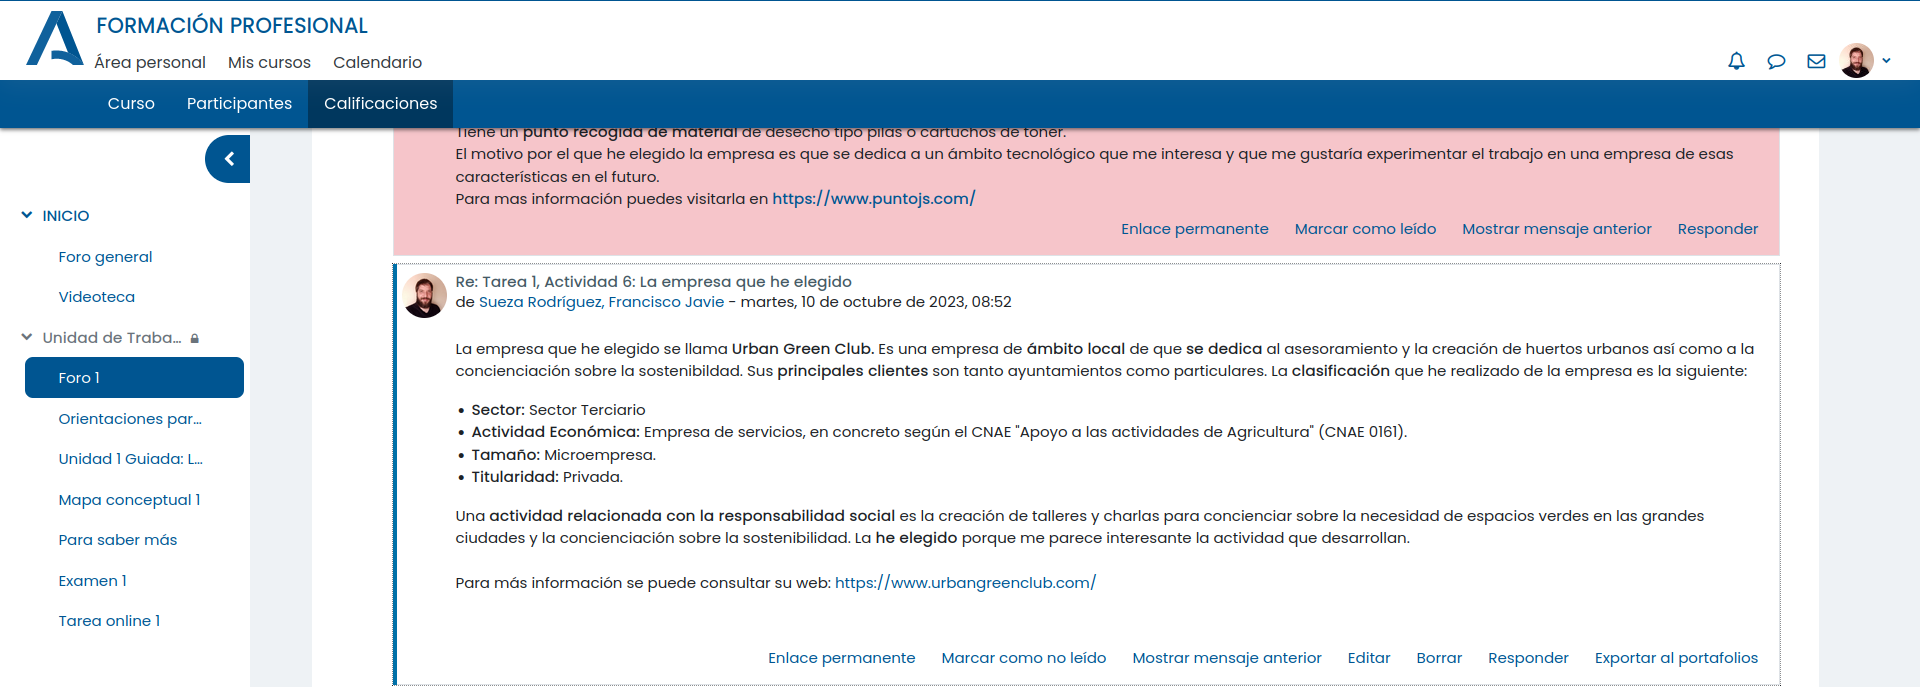
\includegraphics[scale=0.30]{captura-foro.png}
    \caption{Captura del hilo La empresa que he elegido}
\end{figure}

\section{La Empresa y el Entorno}

\subsection{Enunciado}
En el foro de esta unidad encontrarás un hilo que se llama: “Las empresas de mi localidad”.

Participa en el mismo e indica:

\begin{enumerate}
    \item Cuál es tu localidad
    \item Pon un ejemplo de cómo las empresas, con sus buenas o malas prácticas, repercuten en tu entorno.
    \item Relaciona esa situación con los Objetivos de Desarrollo Sostenible (ODS) de la Organización de Naciones Unidas.
\end{enumerate}

Incluye obligatoriamente en este apartado una captura de pantalla de tu intervención para facilitar su corrección.

\textbf{Orientaciones}: investiga en Internet, consulta en los medios de comunicación locales, pregunta en el ayuntamiento, observa…. Recuerda que debe tratarse de un problema de tu localidad.

\subsection{Solución}

% Bibliography

\newpage
\bibliography{citas}
\bibliographystyle{unsrt}

\end{document}